\section{Detecci\'on de ca\'idas}

Para poder detectar una posible caída del robot se cuenta con el giroscopio Gyro, incluido en el kit Bioloid de Robotis. Este giroscopio brinda información sobre la velocidad angular en dos ejes como se muestra en la figura ~\ref{fig:gyroDireccion} . El utilizado en este proyecto es el eje $x$ que indica si el robot experimenta una velocidad hacia adelante o hacia atras. Con esto se puede tener un indicio de si ha caído boca abajo o boca arriba.   

\begin{figure}[hbtp]
\centering
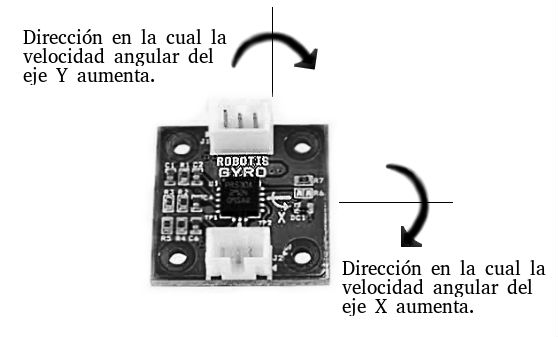
\includegraphics[scale=0.1]{imagenes/gyroDireccion.jpg}
\caption{Dirección en la que la velocidad angular de los ejes $X$ y $Y$, del Gyro, aumenta.}
\label{fig:gyroDireccion}
\end{figure}